\documentclass[justified, openany]{tufte-book}

\usepackage[utf8]{inputenc}
\usepackage[english]{babel}
\usepackage{blindtext}
\usepackage{todonotes}

\setcounter{secnumdepth}{1}
\setcounter{tocdepth}{1}

% turn on numbering for parts and chapters

\usepackage{amsthm, amsmath, amssymb}
\usepackage{setspace, graphicx, enumerate}

\usepackage{stmaryrd}

% For nicely typeset tabular material
\usepackage{booktabs}

\usepackage{listings}
\lstloadlanguages{Haskell}

\usepackage{permute}

\newcommand{\monthyear}{%
  \ifcase\month\or January\or February\or March\or April\or May\or June\or
  July\or August\or September\or October\or November\or
  December\fi\space\number\year
}

% For graphics / images
\usepackage{graphicx}
\usepackage{fancyvrb}
\fvset{fontsize=\normalsize}
\usepackage{xspace}

\usepackage{pgf, tikz}
\usetikzlibrary{arrows,automata,decorations.pathmorphing,backgrounds,positioning,fit,petri,shapes.geometric,calc}

\usepackage{units}

\usepackage{bibentry}

\usepackage{tcolorbox}

\usepackage{enumitem}

\usepackage{bm}

\usepackage{mmacells}

\usepackage{oplotsymbl}

\usepackage{pdfpages}

\usepackage[nottoc]{tocbibind}

\theoremstyle{plain}% default 
\newtheorem{thm}{Theorem}[chapter] 
\newtheorem{lem}[thm]{Lemma} 
\newtheorem{prop}[thm]{Proposition} 
\newtheorem*{cor}{Corollary} 

\theoremstyle{definition} 
\newtheorem{defn}[thm]{Definition}
\newtheorem{conj}[thm]{Conjecture}
\newtheorem{exmp}[thm]{Example}
\newtheorem{exer}[thm]{Exercise}

\newtheorem{proofpart}{Proof Part}[thm]

\theoremstyle{remark} 
\newtheorem*{rem}{Remark} 
\newtheorem*{note}{Note} 
\newtheorem{case}{Case}
\newtheorem{thminv}{Invariant}[chapter] 


\newtcolorbox{problem}{title={Problem}}

\newenvironment{dedication}
    {\vspace{6ex}\begin{quotation}\begin{center}\begin{em}\begin{large}}
    {\par\end{large}\end{em}\end{center}\end{quotation}}

\mmaDefineMathReplacement[≤]{<=}{\leq}
\mmaDefineMathReplacement[≥]{>=}{\geq}
\mmaDefineMathReplacement[≠]{!=}{\neq}
\mmaDefineMathReplacement[→]{->}{\to}[2]
\mmaDefineMathReplacement[⧴]{:>}{:\hspace{-.2em}\to}[2]
\mmaDefineMathReplacement{∉}{\notin}
\mmaDefineMathReplacement{∞}{\infty}
\mmaDefineMathReplacement{𝕕}{\mathbbm{d}}


\mmaSet{
  morefv={gobble=2},
  linklocaluri=mma/symbol/definition:#1,
  morecellgraphics={yoffset=1.9ex}
}



\title{Math notes - Twelve Coins}
\author{Uwe Hoffmann}
\hypersetup{colorlinks, pdftitle={Math notes - Twelve Coins}}

\begin{document}

\setcounter{chapter}{1}
\section*{Twelve Coins}

\newthought{Coin weighings} are the topics of the problem \footnote{\bibentry{Canin94} \\ or \\ Problem 1-111. on page 47 in \bibentry{loehr2017combinatorics}} in this note.\index{coin weighings}

\vspace{10 mm}
\begin{problem}
Of twelve coins, one is counterfeit and weighs either more or less than all the others. The others weigh the same. With a balance scale, on which one side may be weighed against the other, you are to use only three weighings to determine the counterfeit and its type (lighter or heavier). 
\end{problem}

We first present a hand-tailored solution for twelve coins.

Let $M$ be the set of coins, $|M|=12$. We have weighing function
\[
 	w : M \rightarrow \{a, b\},\  a \neq b,\ a, b \in \mathbb{R}^+.
\]

\noindent We have $| \{ c \in M : w(c) = a \} | = 11$ and  $| \{ c \in M : w(c) = b \} | = 1$. We are asked to find 
$c_f \in M$ with $w(c_f) = b$ in three weighings.\bigskip

\noindent For a subset $S \subseteq M$ we define
\[
	w(S) = \sum_{c \in S} w(c).
\]

\begin{marginfigure}

\includegraphics[scale=0.50]{coins.png}
\end{marginfigure}
\marginnote{There are many variations of coin weighing problems. Some require identifying the type of the counterfeit (lighter or heavier), some don't. Some have more than one scale, some have more than one counterfeit, some don't state the existence of the counterfeit, some allow using scale weights or a known genuine coin. The Wikipedia page \url{https://en.wikipedia.org/wiki/Balance_puzzle} has a good overview. In this section we always want to find the counterfeit coin (we know there is exactly one counterfeit of unknown type) and its type and our scale is a balance scale with coins on both sides.}

\noindent Let's partition M into 3 subsets $S_0, S_1, S_2$
\[
	\begin{array}{l}
		S_0 \cup S_1 \cup S_2 = M \\
		\forall \ 0 \leq i < 3 : | S_i | = 4 \\
		\forall \ 0 \leq i <  j < 3 : S_i \cap S_j = \emptyset
	\end{array}	 	
\]

\noindent At this point we consume the first weighing:
\begin{center} \textbf{\textit{1st weighing}}: compare $w(S_1)$ with $w(S_2)$ \end{center}

\subsection{Case $w(S_1) = w(S_2)$}

In this case $c_f \in S_0$. We partition $S_0$ into $S_0 = S_0^1 \cup S_0^3$ with $| S_0^1 | = 1$ and 
$| S_0^3 | = 3$. We also consider $S_1^3$, a subset of $S_1$ with $| S_1^3 | = 3$. We consume the second weighing:
\begin{center} \textbf{\textit{2nd weighing}}: compare $w(S_0^3)$ with $w(S_1^3)$ \end{center}

\begin{description}
	\item [ subcase 1: $w(S_0^3) = w(S_1^3)$. ] In this subcase $c_f \in S_0^1$ and we're done after just two weighings.
	\item [ subcase 2: $w(S_0^3) > w(S_1^3)$. ] In this subcase $S_0^3$ has the counterfeit coin and $b > a$. We consume the third weighing: Let $S_0^3 = \{ c_1, c_2, c_3 \}$. We weigh $c_1$ against $c_2$.
\begin{center} \textbf{\textit{3rd weighing}}: compare $w(c_1)$ with $w(c_2)$ \end{center}
If $w(c_1) = w(c_2)$ then $c_f = c_3$, if $w(c_1) > w(c_2)$ then $c_f = c_1$.
	\item	[ case 3: $w(S_0^3) < w(S_1^3)$. ]  In this case $S_0^3$ has the counterfeit coin and $b < a$. Analog to previous case (replace heavy with light).
\end{description}

\subsection{Case $w(S_1) > w(S_2)$}

In this case the counterfeit coin is either in $S_1$ or in $S_2$.

\begin{marginfigure}[0.0in]
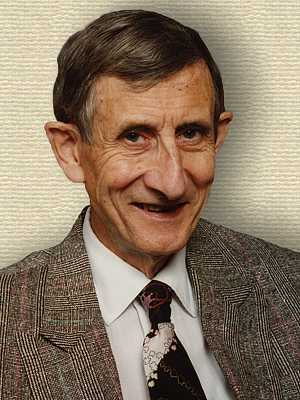
\includegraphics[scale=0.5]{freeman.jpg}
\end{marginfigure}
\marginnote{Freeman J. Dyson. \url{https://en.wikipedia.org/wiki/Freeman_Dyson}}

\noindent We consider 4 subsets:

\begin{description}
	\item $S_0^3 \subset S_0, |S_0^3| = 3$,
	\item $A$ with three coins from $S_1$,
	\item $B$ with one coin from $S_2$,
	\item $C$ with remaining coin from $S_1$: $C = S_1 \setminus A$.
\end{description}
	
\noindent We consume the second weighing:
\begin{center} \textbf{\textit{2nd weighing}}: compare $w(S_0^3 \cup C)$ with $w(A \cup B)$ \end{center}

\begin{description}
	\item [ subcase 1: $w(S_0^3 \cup C) = w(A \cup B)$. ] In this subcase $c_f \in S_2 \setminus B$ and because $w(S_1) > w(S_2)$  we know that $b < a$. Let $\{c_1, c_2, c_3\} = S_2 \setminus B$ and we consume third weighing:
\begin{center} \textbf{\textit{3rd weighing}}: compare $w(c_1)$ with $w(c_2)$ \end{center}
If $w(c_1) = w(c_2)$ then $c_f = c_3$, if $w(c_1) > w(c_2)$ then $c_f = c_2$.	
	\item [ subcase 2: $w(S_0^3 \cup C) < w(A \cup B)$. ] Assume $c_f \in C \subset S_1$. That would mean that $b > a$ because $w(S_1) > w(S_2)$ but that contradicts with \newline
	$w(S_0^3 \cup C) = 3 a + b < w(A \cup B) = 4 a$. Assume $c_f \in B \subset S_2$. That would mean that $b < a$ because $w(S_1) > w(S_2)$ but that contradicts also with
	$w(S_0^3 \cup C) = 4 a < w(A \cup B) = 3 a + b$. The only possibility remaining is $c_f \in A$. We
	use the \textbf{\textit{third weighing}} analog to the previous case to find the counterfeit coin in a three-coin set using the fact that $b > a$.
	\item	[ subcase 3: $w(S_0^3 \cup C) > w(A \cup B)$. ]  In this case the counterfeit coin can be either in $B$ or in $C$. It cannot be in $A$ according to a reasoning analog to previous case that leads to a contradiction. Both $B$ and $C$ only have one coin each so compare the coin in $B$ with any good coin to find the counterfeit coin in this \textbf{\textit{third weighing}}.
\end{description}
	
\noindent This covers all the cases and we're done.

The solution brings up questions: how would it work for 13 coins and in general, how many weighings would be necessary for $N$ coins. To answer these questions we present an elegant general solution\footnote{\bibentry{freemanDysonCoins} \\ We follow an exposition of this solution by G. Shestopal.} invented by Freeman J. Dyson.

In the hand-tailored solution for twelve coins we kept seeing a partition of coin sets into 3 subsets, two equally sized subsets that were weighed against each other and one subset that didn't participate in the current weighing. Depending on the result of the weighing and prior information from previous weighings we could narrow the search. Each weighing seems to contribute roughly three pieces of "information". A sequence of $n$ weighings would generate $3^n$ amount of information that should somehow map to finding the counterfeit amongst $N$ coins. This is not strictly accurate\footnote{The hand-tailored solution is an \textbf{adaptive} solution: later weighings are set up according to the result of earlier weighings. Freeman J. Dyson's general solution is a \textbf{non-adaptive} solution if the number of coins is divisible by three: all the weighings are pre-determined regardless of their outcome.} because information deduced from weighings uses prior information from weighings before and the narrowing doesn't completely discard sets of coins but instead uses them as scale weights with known type (ie none are counterfeits). But this $3^n$ observation does suggest $3^n \approx N$ and point to the objective of finding a bijection between ternary codewords of length $n$ and a set of size $N$. 

Lets first consider $N$ coins with $N$ of the form $N = \frac{1}{2} (3^n - 3)$ for some $n \geq 2$. We will show how to find the counterfeit and its type in $n$ weighings\footnote{Notice that $N=12$ fits this form: $12 = \frac{1}{2} (3^3 - 3)$, so $n=3$ weighings.}.

The set of codewords of length $n$ from alphabet $\{0, 1, 2\}$ has size $3^n$. We discard the three codewords with all digits equal: $0\ldots0$, $1\ldots1$ and $2\ldots2$. The set $W$ of the remaining codewords has size $3^n - 3$. We split\footnote{The expression $3^n - 3$ is the subtraction of two odd numbers, so it is even.} $W$ into $\frac{3^n - 3}{2}$ pairs of complements: 

\begin{defn}
Two codewords $a_1 a_2 \ldots a_n \in W$ and $b_1 b_2 \ldots b_n \in W$ are \textbf{complements} of each other if 
$$
\forall i: 1 \leq i \leq n: a_i + b_i = 2
$$
We use the notation $a_1^c a_2^c \ldots a_n^c$ for the complement of $a_1 a_2 \ldots a_n$.
\end{defn}

\begin{defn}
The function $\delta: W \mapsto \{0, 1, 2\}^2$ finds the first two digits of a codeword that differ\footnote{The function $\delta$ is well-defined because $0\ldots0 \notin W$, $1\ldots1 \notin W$ and $2\ldots2 \notin W$.}
$$
\delta (a_1 a_2 \ldots a_n) = a_i a_{i+1} \text{ such that } \forall 1 \leq j < i: a_j = a_i \text{ and } a_i \neq a_{i+1}
$$
\end{defn}

\begin{defn}
Codeword $w \in W$ is called a \textbf{left} codeword if $\delta(w) \in \{10, 21, 02\}$ otherwise it is called a \textbf{right} codeword. 
\end{defn}
 
It is easy to see that the set of left codewords and the set of right codewords do not overlap and that if a codeword is a left codeword its complement is a right codeword\footnote{For example let's prove that if $a_1 a_2 \ldots a_n$ is a right codeword then $a_1^c a_2^c \ldots a_n^c$ is a left codeword. If $a_j=a_{j+1}$ then $a_j^c=a_{j+1}^c$ and likewise if $a_j \neq a_{j+1}$ then $a_j^c \neq a_{j+1}^c$. So the index of the first two digits that differ is the same for a codeword and its complement. The complements of $\{01, 12, 20\}$ are exactly $\{21, 10, 02\}$ so the complement of a right codeword is a left codeword with differing digits at the same index as the right codeword.}. A good mnemonic of left and right is this: $0 \rightarrow 1 \rightarrow 2$ moves digits to the right so $\{01, 12, 20\}$ corresponds to the right codewords and the right direction. Conversely $0 \leftarrow 1 \leftarrow 2$ moves digits to the left so $\{10, 21, 02\}$ corresponds to the left codewords and the left direction.

To summarize we now have $\frac{3^n - 3}{2}$ pairs of codewords from $W$ such that each pair has a left codeword and a right codeword that are complements of each other. Let $P$ be the set of these pairs. We have $N=\frac{3^n - 3}{2}$ coins. Let $C$ be the set of coins. We pick an arbitrary bijection $\mu: C \mapsto P$ that assigns a pair to a coin, marking it with a left and a right codeword\footnote{For example when $N=12$ we could pick $\mu$ like this:
\begin{center}
\begin{tabular}{ |c|c|c| } 
 \hline
 coin & left codeword & right codeword \\
 \hline
 $c_1$ & $211$ & $011$ \\
 $c_2$ & $100$ & $122$ \\  
 $c_3$ & $022$ & $200$ \\
 $c_4$ & $212$ & $010$ \\
 $c_5$ & $101$ & $121$ \\
 $c_6$ & $020$ & $202$ \\
 $c_7$ & $210$ & $012$ \\
 $c_8$ & $102$ & $120$ \\
 $c_9$ & $021$ & $201$ \\
 $c_{10}$ & $221$ & $001$ \\
 $c_{11}$ & $110$ & $112$ \\
 $c_{12}$ & $002$ & $220$ \\
 \hline
\end{tabular}
\end{center}
$C_3(2)$ means the subset of coins for which the third digit in the right codeword is $2$. In this example $C_3(2) = \{c_2, c_6, c_7, c_{11}\}$.}.

 We adopt the notation $\mu(c).right$ to denote the right codeword assigned to coin $c \in C$ and $\mu(c).left$ the left codeword. Also $\mu(c).right(i)$ denotes the i-th digit of the right codeword, so if $\mu(c).right = a_1 a_2 \ldots a_n$ then $\mu(c).right(i) = a_i$. Analog $\mu(c).left(i)$ for the i-th digit of the left codeword assigned to coin $c$. 

We define $\forall i: 1 \leq i \leq n$ and $\forall d: 0 \leq d \leq 2$ the subsets $C_i(d) \subset C$  with 
$$
C_i(d) = \{ c \in C: \mu(c).right(i) = d\}
$$

It is easy to see that $C = C_i(0) \cup C_i(1) \cup C_i(2)$ for each $1 \leq i \leq n$ and that $C_i(0) \cap C_i(1) = C_i(0) \cap C_i(2) = C_i(1) \cap C_i(2) =\emptyset$, so $C_i(0)$, $C_i(1)$ and $C_i(2)$ partition $C$.

Now we execute $n$ weighings. For the i-th weighing we place the coins from $C_i(0)$ on the left pan of the scale and the coins from $C_i(2)$ on the right pan of the scale. We capture the $n$ weighings in a codeword $x_1 x_2 \ldots x_n \in W$: if in the i-th weighing the left pan sinks, then $x_i=0$, if the weighing is balanced then $x_i=1$ and if the right pan sinks then $x_i=2$. 

We claim that the weighing codeword $x_1 x_2 \ldots x_n$ will be either the left or the right marker codeword of the counterfeit depending whether the counterfeit is lighter or heavier and prove the following theorem:

\begin{thm}\label{coin_encoding}
Let $x_1 x_2 \ldots x_n$ be the result of the $n$ weighings and let $c_f \in C$ be the counterfeit coin.
Then $\mu(c_f).right = x_1 x_2 \ldots x_n$ if $c_f$ is heavier and $\mu(c_f).left = x_1 x_2 \ldots x_n$ if $c_f$ is lighter.
\end{thm}

\begin{proof}
Assume the counterfeit $c_f$ is lighter than the other coins (we deal with the case of $c_f$ heavier afterwards).

There are three cases for the i-th weighing: 

\textbf{Case 1.(lighter)} The scale is balanced, so $x_i=1$. This means that $c_f$ does not participate in the i-th weighing\footnote{Otherwise the scale wouldn't be balanced.}: $c_f \notin C_i(0)$ and $c_f \notin C_i(2)$. Since $C_i(0)$, $C_i(1)$ and $C_i(2)$ partition $C$, we have $c_f \in C_i(1)$. By definition this means that $\mu(c_f).right(i) = x_i = 1$ and since right and left are complements it also means that $\mu(c_f).left(i) = x_i= 1$.

\textbf{Case 2.(lighter)} The left pan sinks, so $x_i=0$. Here $c_f$ participates and $c_f \in C_i(2)$ because it is lighter so on the right pan. By definition this means that $\mu(c_f).right(i) = 2$ and since $\mu(c_f).left(i)$ is the complement it also means $\mu(c_f).left(i) = x_i = 0$.

\textbf{Case 3.(lighter)} The pan sinks, so $x_i=2$. In this case $c_f$ also participates and $c_f \in C_i(0)$ because it is lighter so on the left pan. This means $\mu(c_f).right(i) = 0$ and by complement $\mu(c_f).left(i) = x_i= 2$.
 
For every $i$ we have seen that $\mu(c_f).left(i) = x_i$, so $\mu(c_f).left = x_1 x_2 \ldots x_n$.
 	
Now assume $c_f$ is heavier. We proceed in analog fashion. There are three cases for the i-th weighing:

\textbf{Case 1.(heavier)} The scale is balanced, so $x_i=1$. This means that $c_f$ does not participate in the i-th weighing and we have $c_f \in C_i(1)$ and $\mu(c_f).right(i) = x_i = 1$.

\textbf{Case 2.(heavier)} The left pan sinks, so $x_i=0$. Here $c_f$ participates and $c_f \in C_i(0)$ because it is heavier so on the left pan. Then $\mu(c_f).right(i) = x_i = 0$.

\textbf{Case 3.(heavier)} The right pan sinks, so $x_i=2$. In this case $c_f$ also participates and $c_f \in C_i(2)$ because it is heavier so on the right pan. So $\mu(c_f).right(i) = x_i= 2$.

We see that for every $i$ we have $\mu(c_f).right(i) = x_i$, so $\mu(c_f).right = x_1 x_2 \ldots x_n$.
\end{proof}

Theorem \ref{coin_encoding} shows that the $n$ weighings detect the counterfeit coin and its type if there are $N = \frac{3^n - 3}{2}$ coins.

If $N < \frac{3^n - 3}{2}$ we have to be more careful how we mark coins with codewords\footnote{For example assume there are only ten coins and we arbitrarily assign the following codeword pairs:
\begin{center}
\begin{tabular}{ |c|c|c| } 
 \hline
 coin & left codeword & right codeword \\
 \hline
 $c_1$ & $211$ & $011$ \\
 $c_2$ & $100$ & $122$ \\  
 $c_3$ & $022$ & $200$ \\
 $c_4$ & $212$ & $010$ \\
 $c_5$ & $101$ & $121$ \\
 $c_6$ & $020$ & $202$ \\
 $c_7$ & $210$ & $012$ \\
 $c_8$ & $102$ & $120$ \\
 $c_9$ & $021$ & $201$ \\
 $c_{10}$ & $221$ & $001$ \\
 \hline
\end{tabular}
\end{center}
Then $C_2(2) = \{c_2, c_5, c_8\}$ and $C_2(0) = \{c_3, c_6, c_9, c_{10}\}$. This is a problem because the two sets that will be put on the scale in the two pans in the second weighing have different number of coins. We cannot deduce any information from this weighing anymore.
}.

Let $\pi: W \mapsto W$ be the function on the set of codewords $W$ with $\pi(a_1 a_2 \ldots a_n) = b_1 b_2 \ldots b_n$ such that $\forall i: 1 \leq i \leq n: b_i \equiv (a_i + 1) \mod 2$.

\begin{lem}\label{coin_pi}
The function $\pi$ preserves the rightiness of codewords: if $w \in W$ is a right codeword, then $\pi(w)$ is also a right codeword.
\end{lem}

\begin{proof}
Let $a_1 a_2 \ldots a_n$ be a right codeword. By definition it means that $\delta(a_1 a_2 \ldots a_n)=a_i a_{i+1}$ with $\forall 1 \leq j < i: a_j = a_i$ and $a_i a_{i+1} \in \{01, 12, 20\}$. Let $\pi(a_1 a_2 \ldots a_n) = b_1 b_2 \ldots b_n$. This means that $\forall 1 \leq j < i: b_j \equiv a_j + 1 \equiv a_i + 1 \equiv b_i \mod 2$. So $\delta(b_1 b_2 \ldots b_n) = b_i b_{i+1}$. If $a_i a_{i+1}=01$ then $b_i b_{i+1}=12$, if $a_i a_{i+1}=12$ then $b_i b_{i+1}=20$ and if $a_i a_{i+1}=20$ then $b_i b_{i+1}=01$. In all three cases $b_1 b_2 \ldots b_n$ is also a right codeword.
\end{proof}

From the definition of $\pi$ it is clear that $\pi^3(w) = w$. From this and lemma \ref{coin_pi} it follows that $\pi$ partitions the set of right codewords into subsets of size three: $\{w, \pi(w), \pi^2(w)\}$.

We now partition $W$ into subsets of size six: 
$$
\{w, w^c, \pi(w), (\pi(w))^c, \pi^2(w), (\pi^2(w))^c\}
$$
grouping $\pi$-generated right codewords and their left complements. The group with right codewords $00\ldots01$, $11\ldots12$ and $22\ldots20$ we set aside and call the left-over group. 

For the bijection $\mu: C \mapsto W$ we group coins in groups of three. For each group we pick a codeword group of six other than the left-over group and assign left and right complementing codewords to each coin in the group. If there are one or two coins left over from the grouping into threes, then we use the left-over codeword group to assign left and right codewords to those coins. If only one coin is left over we assign it the right codeword $11\ldots12$ and if two are left over we assign the right codewords $00\ldots01$ and $22\ldots20$.

With $\mu$ defined this way if $N \equiv 1 \mod 3$ then the left-over coin has right codeword $11\ldots12$ and will not participate in the first $n-1$ weighings. If $N \equiv 2 \mod 3$ the two left-over coins with right codewords $00\ldots01$ and $22\ldots20$ will both participate in every of the first $n-1$ weighings. This ensures that the left-over coins don't disrupt the first $n-1$ weighings. For a coin that is not in the left-over group it is easy to see that if it participates in a weighing then there is another coin in the same group (apply $\pi$ twice to get to its right codeword) that also participates on the opposite pan. Overall we have satisfied the requirement $|C_i(0)| = |C_i(2)|$ for all $1 \leq i < n$. The first $n-1$ weighings can proceed as before.

For the last weighing we have the following cases (here the solution turns adaptive, ie the setup for the last weighing depends on the outcome of the previous weighings):

The first two cases are for $N \equiv 1 \mod 3$, so one left-over coin $c_l$ with right codeword $\mu(c_l).right=11\ldots12$. 

\textbf{Case 1.} The first $n-1$ weighings yielded $x_1 x_2 \ldots x_{n-1} = 11\ldots1$ (the scale was balanced in all $n-1$ weighings). In this case we know the left-over coin is the counterfeit $c_l=c_f$ and we can just put it on one pan on the scale and any other coin on the other to determine its type.

\textbf{Case 2.} The first $n-1$ weighings yielded $x_1 x_2 \ldots x_{n-1} \neq 11\ldots1$. In this case we know the left-over coin is not the counterfeit. We can just leave it out and put $C_n(0)$ on the left pan and $C_n(2) \setminus \{c_l\}$ on the right pan of the balance scale. The resulting complete weighing codeword will point to the counterfeit and its type.

The next cases are for for $N \equiv 2 \mod 3$, with two left-over coins $c_{l0}$ and $c_{l2}$ with right codewords $\mu(c_{l0}).right=00\ldots01$ and $\mu(c_{l2}).right=22\ldots20$.

\textbf{Case 3.} The first $n-1$ weighings yielded $x_1 x_2 \ldots x_{n-1} = 22\ldots2$. Both $c_{l0}$ and $c_{l2}$ participated in all $n-1$ weighings (according to their right codewords that start with $00\ldots0$ and $22\ldots2$ respectively). It means that either $c_{l0}$ or $c_{l2}$ is the counterfeit.  In the last weighing we pit $c_{l0}$ against any coin that is not $c_{l2}$. If the scale is balanced then $c_{l2}$ is the counterfeit and it is heavier. If the scale tilts one way or the other it shows $c_{l0}$ as a counterfeit and its type.

\textbf{Case 4.} The first $n-1$ weighings yielded $x_1 x_2 \ldots x_{n-1} = 00\ldots0$. Again both $c_{l0}$ and $c_{l2}$ participated in all $n-1$ weighings and again it means that either $c_{l0}$ or $c_{l2}$ is the counterfeit.  In the last weighing we pit $c_{l2}$ against any coin that is not $c_{l0}$. If the scale is balanced then $c_{l0}$ is the counterfeit and it is heavier. If the scale tilts one way or the other it shows $c_{l2}$ as a counterfeit and its type.

\textbf{Case 5.} The first $n-1$ weighings yielded $x_1 x_2 \ldots x_{n-1} \neq 00\ldots0$ and $x_1 x_2 \ldots x_{n-1} \neq 22\ldots2$. In this case both $c_{l0}$ and $c_{l2}$ cannot be counterfeits. In the last weighing we can just do $C_n(0)$ on the left pan and $C_n(2)$ on the right. The resulting complete weighing codeword will point to the counterfeit and its type.

This covers all the cases and shows that we can find the counterfeit coin and its type in $n$ weighings if the number of coins $N \leq \frac{3^n - 3}{2}$. 

Is this optimal or does a strategy exist that needs less than $n$ weighings?

To answer this question we want to find a lower bound for the number of weighings given $N$ coins.  

\begin{thm}\label{coin_lower_bound}
Given are $N$ coins of which one is a counterfeit. If the counterfeit coin and its type can be found in $n$ weighings using a non-adaptive strategy, then $2 N \leq 3^n - 3$.
\end{thm}

\begin{proof}

There are $n$ weighings producing a weighing codeword $x_1 x_2 \ldots x_n$ with $x_i=0$ if left pan sinks in i-th weighing, $x_i=1$ if i-th weighing is balanced and $x_i=2$ if right pan sinks. We have $3^n$ possible codewords from $n$ weighings.

Assume we have a non-adaptive strategy that finds the counterfeit coin and its type in $n$ weighings. Since it is non-adaptive the information of which coin participates in which weighing on which pan is already pre-determined. Let's capture this information in a matrix $p \in \{0, 1, 2\}^{n \times N}$ which we call the \textbf{participation matrix}:

$$
\begin{array}{l}
\forall 1 \leq i \leq n, 1 \leq j \leq N: \\
p_{ij} = 
\begin{cases}
0 \text{,  \quad  coin $j$ on left pan in i-th weighing} \\
1 \text{,  \quad  coin $j$ not in i-th weighing} \\
2 \text{,  \quad  coin $j$ on right pan in i-th weighing}
\end{cases}
\end{array}
$$

The number of potential answers to the question of which coin is the counterfeit and what is its type is $2 N$ ($N$ coins and two possibilities for each coin - lighter or heavier). For notational convenience we define the index sequence $N_{\pm} = \{1, -1, 2, -2, \ldots , N, -N\}$. For all $1 \leq j \leq N$ index $j$ means coin $j$ is the counterfeit and it is heavier, index $-j$ means coin $j$ is the counterfeit and it is lighter.

Given the participation matrix we define a matrix $a \in \{0, 1, 2\}^{n \times N_{\pm}}$. Cell $a_{ij}$ tells us what result of weighing $i$ keeps the answer that coin $j$ is the heavier counterfeit as still a possibility. Cell $a_{i(-j)}$ tells us what result of weighing $i$ keeps the answer that coin $j$ is the lighter counterfeit as still a possibility. For example if $p_{ij} = 0$ then coin $j$ is on the left pan in the i-th weighing and for coin $j$ to be the counterfeit and heavier in the i-th weighing the left pan needs to sink, the corresponding weighing codeword component needs to be $x_i=0$ and $a_{ij} = 0$.

In other words matrix $a$ shows for each potential answer what needs to happen in each weighing so that the answer becomes the actual answer:

$$
\begin{array}{l}
\forall 1 \leq i \leq n, 1 \leq j \leq N: \\
a_{ij} = 
\begin{cases}
0  \text{,\quad if } p_{ij} = 0\\
1  \text{,\quad if } p_{ij} = 1\\
2  \text{,\quad if } p_{ij} = 2
\end{cases}
a_{i(-j)} = 
\begin{cases}
0  \text{,\quad if } p_{ij} = 2\\
1  \text{,\quad if } p_{ij} = 1\\
2  \text{,\quad if } p_{ij} = 0
\end{cases}
\end{array}
$$

The column $j$ in matrix $a$ is the weighing codeword required for making coin $j$ and its type (from the sign of $j$) the actual answer.

For the strategy (represented by the participation matrix $p$) to work it needs to not rely on "luck", i.e.\ a given weighing codeword happens to be a column in matrix $a$. All the weighing codewords that can occur need to be columns in $a$ exactly once. 

Since the strategy is successful we know that each coin participates in at least one weighing\footnote{Otherwise there would be no way to find its type even if we find the counterfeit.}, so the column vector $(1, 1, \ldots, 1)^T$ does not appear in $p$. This means that weighing codeword $x1 x2 \ldots x_n=11\ldots1$ cannot occur and we have $3^n - 1$ remaining weighing codewords that can happen.

If $2 N > 3^n - 1$ then it must be that a weighing codeword will appear more than once in $a$, so more than one potential answer could be the actual answer and we wouldn't know which one. So $2 N \leq 3^n - 1$.

We observe that in each row $i$ of $a$ if $a_{ij}=0$ then $a_{i(-j)}=2$ and vice versa. That means that there are $k_i$ zeros and $k_i$ twos in row $i$, so $2 N - 2 k_i$ ones. Also because an even number of coins participates in each weighing we have that $k_i$ is even. So in each row we have an even number of zeros, ones and twos. There are $3^{n - 1}$ possible weighing codewords that start with a one. That means at most $3^{n-1}$ columns in $a$ can have a one in the first position. Since the number of ones is even and $3^{n-1}$ is odd we can have at most $3^{n-1}-1$ ones in the first row. Similarly there are $3^{n - 1}$ possible weighing codewords that start with a zero, so $k_1 \leq 3^{n-1} - 1$. We then have:

$$
2N = 2N - 2 k_1 + 2 k_1 \leq 3^{n-1} - 1 + 2 (3^{n-1} - 1) = 3^n - 3    
$$
\end{proof}

\todo{Explain connection to Hamming codes for number of columns smaller than $3^n - 3$}

\bibliographystyle{plainnat}
\bibliography{../common/math}

\end{document}
